\begin{frame} %=================================================================
  \frametitle{The specifics: Contents}

  \begin{wideitemize}
    \item Terminology - Notation
    \item Problem
    \item Solutions
    \item Simulations
  \end{wideitemize}

\end{frame} %-------------------------------------------------------------------
\note{OK so next I'll talk about the problem and start formalizing it}
%###############################################################################
%###############################################################################
%###############################################################################
%###############################################################################
\begin{frame} %=================================================================
  \frametitle{Model in Space}

\begin{figure}[H]\centering
  \scalebox{0.8}{\begin{tikzpicture}[scale = 0.5]
	%draw the global frame
	\draw [color=black,thick,->,>=stealth'](-12, -5) to (-7, -5);
	\draw [color=black,thick,->,>=stealth'](-12, -5) to (-12, -3);
	\draw [color=black,thick,->,>=stealth'](-12, -5) to (-10, -6.5);
  \node at (-12.9, -5.0) {$\{\mathcal{O}\}$};

	%draw agent i
	\draw [color = blue, fill = blue!20] (-4.5,0) circle (2.5cm);
  \node at (-5.7, -0.2) {$\{i\}$};
	\draw[green,thick,dashed] (-4.5,0) circle (6.0cm);
	\draw [color=black,thick,->,>=stealth'](-12, -5) to (-4.5, -0.1);
	\node at (-7.7, -1.5) {$p_i$};
	\draw [color=green,thick,dashed,->,>=stealth'](-4.5, 0.0) to (-9.93, 2.43);
	\node at (-8.3, 2.15) {$d_i$};
	\draw [color=black,thick,dashed,->,>=stealth'](-4.5, 0.0) to (-2.0, 0.0);
	\node at (-3.3, 0.3) {$r_i$};
	\node at (-4.5, 0.0) {$\bullet$};
	\node at (-5.8, 3.0) {$\mathcal{B}(p_i, r_i)$};

	%draw agent j
	\draw [color = red, fill = red!20] (0.2, 0) circle (1.5cm);
	\node at (-0.5, 0.3) {$\{j\}$};
	\draw[orange,thick,dashed,] (0.2, 0) circle (5.1cm);
	\draw [color=black,thick,->,>=stealth'](-12, -5) to (0.2, -0.1);
	\node at (-6.0, -3.2) {$p_j$};
	\draw [color=orange,thick,dashed,->,>=stealth'](0.2, 0.0) to (5.2, -1.0);
	\node at (3.8, -0.1) {$d_j$};
	\draw [color=black,thick,dashed,->,>=stealth'](0.2, 0.0) to (1.7, 0.0);
	\node at (1.1, 0.3) {$r_j$};
	\node at (0.2, 0.0) {$\bullet$};
	\node at (0.68, -2.1) {$\mathcal{B}(p_j, r_j)$};

\end{tikzpicture}
}
  \caption{Agents $i$, $j$: spherical rigid bodies with radii $r_i > r_j$.
    Vectors $p_i$, $p_j$ show center mass positions. $d_i > d_j$ are their sensing
    ranges.}
  \label{}
\end{figure}

\end{frame} %-------------------------------------------------------------------
\note{We model agents in space as spherical rigid bodies, of radius $r$,
  which have a limited connectivity range of $d$, moving in space with
  $p$ denoting their position through time.}
%###############################################################################
%###############################################################################
%###############################################################################
%###############################################################################
\begin{frame} %=================================================================
  \frametitle{Dynamics}

  Agents $i \in \mathcal{V} = \{1,2,\dots,N\}$, with radii $r_i$ and ranges $d_i$\\[4ex]

  Each agent $i\in\mathcal{V}$ is described by a continuous-time non-linear model

  \begin{align}
    \dot{\vect{x}}_i = f_i(\vect{x}_i, \vect{u}_i) + \vect{\delta}_i
  \end{align}

  $\vect{x}_i \in X_i$, $\vect{u}_i \in U_i$\\[4ex]

  with \textit{unknown} disturbance
  $\vect{\delta}_i \in \Delta_i : \|\vect{\delta}_i\|_{\infty} = \overline{\delta}_i$

\end{frame} %-------------------------------------------------------------------
\note{In terms of dynamics, all agents are described by continuous-time, non-linear
  differential equations that include additive and bounded disturbance terms that
  are unknown.}
%###############################################################################
%###############################################################################
%###############################################################################
%###############################################################################
\begin{frame} %=================================================================
  \frametitle{Solution requirements (0/III)}

  Design decentralized control policies $\vect{u}_i \in \mathcal{U}_i$ such that\\[3ex]

  \begin{ww_box}
  \begin{wideitemize}

    \item<2-> Collisions are avoided for all\ \ $i,j \in \mathcal{V}$,\ \ $\ell \in \mathcal{L}$,\ \ $t \geq 0$
      \begin{align}
        \|\vect{p}_i(t) - \vect{p}_{j}(t)\| > \underline{d}_{ij,a} \\
        \|\vect{p}_i(t) - \vect{p}_\ell\| > \underline{d}_{i\ell,o}
      \end{align}

      $\vect{p}_i$ component of state $\vect{x}_i$\\[3ex]

    \item<2-> Neighbours $i \in \mathcal{N}_j$, $j \in \mathcal{N}_i$
      maintain connectivity at all times $t \geq 0$
      \begin{align}
        \|\vect{p}_i(t) - \vect{p}_{j}(t)\| < \text{min}(\overline{d}_{i}, \overline{d}_{j})
      \end{align}
  \end{wideitemize}
  \end{ww_box}

  \begin{wideitemize}
    \item<3-> (Closed-loop) System is stable at desired state
      \begin{align}
        \lim\limits_{t \to \infty}\|\vect{x}_i(t) - \vect{x}_{i,\text{des}}\| \to 0 \\
      \end{align}

  \end{wideitemize}

\end{frame} %-------------------------------------------------------------------
\note{Formally then, the problem lies in designing a control regime such that
  all input signals stay bounded, no collisions occur, all neighbours
  stay well-connected at all times, and that all agents are stabilized in
  steady-state}
%###############################################################################
%###############################################################################
%###############################################################################
%###############################################################################
\begin{frame} %=================================================================
  \frametitle{Solution requirements (I/III): constraint design}

  Design decentralized control policies $\vect{u}_i \in \mathcal{U}_i$ such that\\[3ex]

  \begin{gg_box}
  \begin{wideitemize}

    \item Collisions are avoided for all\ \ $i,j \in \mathcal{V}$,\ \ $\ell \in \mathcal{L}$,\ \ $t \geq 0$
      \begin{align}
        \|\vect{p}_i(t) - \vect{p}_{j}(t)\| > \underline{d}_{ij,a} \\
        \|\vect{p}_i(t) - \vect{p}_\ell\| > \underline{d}_{i\ell,o}
      \end{align}

      $\vect{p}_i$ component of state $\vect{x}_i$\\[3ex]


    \item Neighbours $i \in \mathcal{N}_j$, $j \in \mathcal{N}_i$
      maintain connectivity at all times $t \geq 0$
      \begin{align}
        \|\vect{p}_i(t) - \vect{p}_{j}(t)\| < \text{min}(\overline{d}_{i}, \overline{d}_{j})
      \end{align}
  \end{wideitemize}
  \end{gg_box}


  \begin{wideitemize}
    \item (Closed-loop) System is stable at desired state
      \begin{align}
        \lim\limits_{t \to \infty}\|\vect{x}_i(t) - \vect{x}_{i,\text{des}}\| \to 0 \\
      \end{align}

  \end{wideitemize}

\end{frame} %-------------------------------------------------------------------
\note{I will first focus on the second requirement and then go through the other two.}
%###############################################################################
%###############################################################################
%###############################################################################
%###############################################################################
\begin{frame} %=================================================================
  \frametitle{State constraint set}

  Encode all state requirements on agent $i$ through time-varying set $\mathcal{Z}_i$.

  \begin{align}
    \mathcal{Z}_i = \{ \vect{x}_i(t) \in X_i :
        &\|\vect{p}_i(t) - \vect{p}_{j}(t)\| > \underline{d}_{ij,a},\ \ \forall j \in \mathcal{R}_i(t), \\[2ex]
        &\|\vect{p}_i(t) - \vect{p}_{j}(t)\| < \overline{d}_{i},\ \ \ \ \ \forall j \in \mathcal{N}_i, \\[2ex]
        &\|\vect{p}_i(t) - \vect{p}_\ell\| > \underline{d}_{i\ell,o},\ \ \ \ \ \ \forall \ell \in \mathcal{L} \}
  \end{align}

  $\mathcal{R}_i(t)$: agents within range of agent $i$ at time $t$

  $\mathcal{N}_i$: assigned neighbours of agent $i$\\[4ex]

  The problem requires $\vect{x}_i(t) \in \mathcal{Z}_i$ for $t \geq 0$

\end{frame} %-------------------------------------------------------------------
\note{The good thing with MPC as I mentioned is that we can encode all
  constraints in a set, say Z, which in our case is time-varying. The problem
  merely requires that the trajectories of each agent are kept within Z.}
%###############################################################################
%###############################################################################
%###############################################################################
%###############################################################################
\begin{frame} %=================================================================
  \frametitle{error-wise}

  The \textit{error} of agent $i\in\mathcal{V}$ with respect to $\vect{x}_{i,\text{des}}$
  is
  $$\vect{e}_i(t) = \vect{x}_i(t) - \vect{x}_{i,\text{des}}$$

  Described by a continuous-time non-linear model

  \begin{align}
    \dot{\vect{e}}_i = g_i(\vect{e}_i, \vect{u}_i) + \vect{\delta}_i
  \end{align}
  \begin{align}
    \vect{e}_i &\in \mathcal{E}_i \equiv \mathcal{Z}_i \ominus \vect{x}_{i,\text{des}} \\
    \vect{u}_i &\in U_i \\
    \vect{\delta}_i &\in \Delta_i
  \end{align}

  where $\mat{A} \ominus \vect{b} = \{\vect{a} - \vect{b}, \vect{a} \in \mat{A}\}$
  is the Minkowski (Pontryagin) difference operation

\end{frame} %-------------------------------------------------------------------
\note{If we look at the system in terms of error, we can get its dynamics
and express the corresponding constraint set by using the minkowski set
difference. We will be speaking in terms of error for the following slides.}
%###############################################################################
%###############################################################################
%###############################################################################
%###############################################################################
\begin{frame} %=================================================================
  \frametitle{Solution requirements (II/III): control input}

  \begin{gg_box}
  Design decentralized $\vect{u}_i \in \mathcal{U}_i$ such that
  \end{gg_box}

  \begin{wideitemize}

    \item Collisions are avoided for all\ \ $i,j \in \mathcal{V}$,\ \ $\ell \in \mathcal{L}$,\ \ $t \geq 0$
      \begin{align}
        \|\vect{p}_i(t) - \vect{p}_{j}(t)\| > \underline{d}_{ij,a} \\
        \|\vect{p}_i(t) - \vect{p}_\ell\| > \underline{d}_{i\ell,o}
      \end{align}

      $\vect{p}_i$ component of state $\vect{x}_i$\\[3ex]

    \item Neighbours $i \in \mathcal{N}_j$, $j \in \mathcal{N}_i$
      maintain connectivity at all times $t \geq 0$
      \begin{align}
        \|\vect{p}_i(t) - \vect{p}_{j}(t)\| < \text{min}(\overline{d}_{i}, \overline{d}_{j})
      \end{align}

    \item (Closed-loop) System is stable at desired state
      \begin{align}
        \lim\limits_{t \to \infty}\|\vect{x}_i(t) - \vect{x}_{i,\text{des}}\| \to 0 \\
      \end{align}

  \end{wideitemize}

\end{frame} %-------------------------------------------------------------------
\note{If we now focus on the control input requirements\dots}
%###############################################################################
%###############################################################################
%###############################################################################
%###############################################################################
\begin{frame}
  \frametitle{Solution requirements (II/III): control input}

  Designed control input $\vect{u}_i$ must\\[2ex]

  \begin{wideitemize}
    \item result in states that satisfy the state constraints \\[2ex]
    \item drive trajectory to / stabilize at desired state (how close?) \\[2ex]
    \item exist and be feasible $\forall t \geq 0$ ($\vect{u}_i \in \mathcal{U}_i$) \\[2ex]
  \end{wideitemize}

\end{frame}
\note{\dots Such an input can be obtained by solving an optimization problem
  at regular sampling intervals.}
%###############################################################################
%###############################################################################
%###############################################################################
%###############################################################################
\begin{frame} %=================================================================
  \frametitle{The optimization problem}

\begin{align}
  \text{Given }& \text{measurement } \vect{e}_i(t_k), \text{find} \\[2ex]
              &\overline{\vect{u}}_i^{\star} (\cdot;\ \vect{e}_i(t_k)) \triangleq \text{argmin }\limits_{\overline{\vect{u}}_i (\cdot)}\
    J_i \big(\vect{e}_i(t_k), \overline{\vect{u}}_i (\cdot) \big) \label{position_based_cost_2} \\[2ex]
    \text{where}& \\
    &J_i \big(\vect{e}_i(t_k), \overline{\vect{u}}_i (\cdot) \big) \triangleq
      \int_{t_k}^{t_k + T_p} F_i \big(\overline{\vect{e}}_i(s), \overline{\vect{u}}_i (s)\big) ds \ + \
      V_i \big(\overline{\vect{e}}_i (t_k + T_p)\big)  \\
  \text{subject to:} & \nonumber \\
                     & \dot{\overline{\vect{e}}}_i(s) = g_i \big(\overline{\vect{e}}_i (s), \overline{\vect{u}}_i (s)\big) \label{eq:internal_error_model_2},
                       \quad \overline{\vect{e}}_i (t_k) = \vect{e}_i (t_k) \\[2.5ex]
                     & \overline{\vect{u}}_i(s) \in \mathcal{U}_i,
                       \quad \overline{\vect{e}}_i (s) \in \mathcal{E}_{i, s - t_k},
                       \quad s \in [t_k, t_k + T_p]\\[2.5ex]
                     & \overline{\vect{e}}_i (t_k + T_p) \in \Omega_i
\end{align}
\end{frame} %-------------------------------------------------------------------
\note{it is the input that minimizes a standard MPC
criterion over a period of $T_p$ time units. This is the
typical formulation of the MPC solution. However, there is
a big difference here. The disturbance is unaccounted
for in the dynamics of the solution because it is unknown.}
%###############################################################################
%###############################################################################
%###############################################################################
%###############################################################################
\begin{frame} %=================================================================
  \frametitle{Issue \#1}

  The disturbance is unknown to the controller. \\[4ex]
  \textbf{How can we guarantee that } $\vect{e}_i \in \mathcal{E}_i$ ? \\[6ex]

  Somehow the disturbance needs to be accounted for within the optimization problem.


\end{frame} %-------------------------------------------------------------------
\note{And so the first question we are asking is: how can we guarantee that
the error does not escape the set in which we want it to be?}
%###############################################################################
%###############################################################################
%###############################################################################
%###############################################################################
\begin{frame} %=================================================================
  \frametitle{The optimization problem}

\begin{align}
  \text{Given }& \text{measurement } \vect{e}_i(t_k), \text{find} \\[2ex]
              &\overline{\vect{u}}_i^{\star} (\cdot;\ \vect{e}_i(t_k)) \triangleq \text{argmin }\limits_{\overline{\vect{u}}_i (\cdot)}\
    J_i \big(\vect{e}_i(t_k), \overline{\vect{u}}_i (\cdot) \big) \label{position_based_cost_2} \\[2ex]
    \text{where}& \\
    &J_i \big(\vect{e}_i(t_k), \overline{\vect{u}}_i (\cdot) \big) \triangleq
      \int_{t_k}^{t_k + T_p} F_i \big(\overline{\vect{e}}_i(s), \overline{\vect{u}}_i (s)\big) ds \ + \
      V_i \big(\overline{\vect{e}}_i (t_k + T_p)\big)  \\
  \text{subject to:} & \nonumber \\
                     & \dot{\overline{\vect{e}}}_i(s) = g_i \big(\overline{\vect{e}}_i (s), \overline{\vect{u}}_i (s)\big) \label{eq:internal_error_model_2},
                       \quad \overline{\vect{e}}_i (t_k) = \vect{e}_i (t_k) \\[2.5ex]
                     & \overline{\vect{u}}_i(s) \in \mathcal{U}_i,
                       \quad \mymkellipse{\overline{\vect{e}}_i (s) \in \mathcal{E}_{i, s - t_k}},
                       \quad s \in [t_k, t_k + T_p]\\[0.5ex]
                     & \overline{\vect{e}}_i (t_k + T_p) \in \Omega_i
\end{align}
\end{frame} %-------------------------------------------------------------------
\note{What we do in this case is manipulate the set in which the error should
lie in within the solution of the optimization problem. And that is what this
(shows red) constraint is.  At each step we progressively tighten the
original constraint set during the solution of the optimization problem, so
that, irrespective of the actual magnitude of the disturbance affecting the
real system, its real trajectory always stays within the prescribed constraints.
And we can do this because we know the supremum of the disturbance}

%###############################################################################
%###############################################################################
%###############################################################################
%###############################################################################
\begin{frame} %=================================================================
  \frametitle{Restricted constraint set (1/5)}

  %Luckily we know $\overline{\delta}_i$

  $\mathcal{E}_{i, s-t_k} \equiv \mathcal{E}_i \ominus \mathcal{B}_{i,s-t_k}$ \\[2ex]
  $\mathcal{B}_{i,s-t_k} \equiv \{\overline{\vect{e}}_i: \|\overline{\vect{e}}_i\| \leq \zeta(\overline{\delta}_i, s)\}$,\ \
  $\zeta(\nearrow, \nearrow)$

\begin{figure}
  \scalebox{0.55}{\begin{tikzpicture}[scale = 1, rotate=-30]
  \draw (2,2) ellipse (6cm and 3cm);
    \node at ($(-3.8,0.8)+(75:6 and 3)$) {$\mathcal{E}_i$};

\pgflowlevel{\pgftransformrotate{30}}
\end{tikzpicture}
}
  \caption{The set where all real trajectories must lie in.}
\end{figure}

\end{frame} %-------------------------------------------------------------------
\note{What is the logic behind this manipulation? Let's depict the real constraint set of the
error with this ellipse. When solving the optimization problem, we consider
the evolution of the trajectory of the error for a number of time units.
If disturbances are present, then, as time goes by, the true state becomes
more and more unpredictable as more and more disturbance has affected it in the
course of time, since the input given to the system does not know anything about
the disturbances. The more time goes by and the more disturbance is present,
the more unpredictable the system becomes, and the more likely it is that its
states will escape the constraint set. If instead we restrict the predicted
trajectory in a reverse manner at each step to be futher and further away from the boundary of the
constraints, then we can guard the system from violating its constraints,
provided that the horizon has been selected so that the last constrained set is
not empty.
}
%###############################################################################
%###############################################################################
%###############################################################################
%###############################################################################
\begin{frame} %=================================================================
  \frametitle{Restricted constraint set (2/5)}

  %Luckily we know $\overline{\delta}_i$

  $\mathcal{E}_{i, s-t_k} \equiv \mathcal{E}_i \ominus \mathcal{B}_{i,s-t_k}$ \\[2ex]
  $\mathcal{B}_{i,s-t_k} \equiv \{\overline{\vect{e}}_i: \|\overline{\vect{e}}_i\| \leq \zeta(\overline{\delta}_i, s)\}$,\ \
  $\zeta(\nearrow, \nearrow)$

\begin{figure}
  \scalebox{0.55}{\begin{tikzpicture}[scale = 1, rotate=-30]
  \draw (2,2) ellipse (6cm and 3cm);
    \node at ($(-3.8,0.8)+(75:6 and 3)$) {$\mathcal{E}_i$};
  \draw[dashed] (2,2) ellipse (5cm and 2.5cm);
    \node at ($(-2.3,1.2)+(75:5 and 2.5)$) {$\mathcal{E}_i \ominus \mathcal{B}_{i,t_{k+1} - t_k}$};

\pgflowlevel{\pgftransformrotate{30}}
\end{tikzpicture}
}
  \caption{The set where all \textit{predicted} trajectories are restricted in, when $t = t_k + h$, dashed.}
\end{figure}

\end{frame} %-------------------------------------------------------------------
\note{In the first step, when $t=t_{k+1}$, the real constraint set is
  reduced to the states that will not violate the constraints if at $t=t_k$
  the disturbance hits its maximum.}
%###############################################################################
%###############################################################################
%###############################################################################
%###############################################################################
\begin{frame} %=================================================================
  \frametitle{Restricted constraint set (3/5)}

  %Luckily we know $\overline{\delta}_i$

  $\mathcal{E}_{i, s-t_k} \equiv \mathcal{E}_i \ominus \mathcal{B}_{i,s-t_k}$ \\[2ex]
  $\mathcal{B}_{i,s-t_k} \equiv \{\overline{\vect{e}}_i: \|\overline{\vect{e}}_i\| \leq \zeta(\overline{\delta}_i, s)\}$,\ \
  $\zeta(\nearrow, \nearrow)$

\begin{figure}
  \scalebox{0.55}{\begin{tikzpicture}[scale = 1, rotate=-30]
  \draw (2,2) ellipse (6cm and 3cm);
    \node at ($(-3.8,0.8)+(75:6 and 3)$) {$\mathcal{E}_i$};
  \draw[dashed] (2,2) ellipse (5cm and 2.5cm);
    \node at ($(-2.3,1.2)+(75:5 and 2.5)$) {$\mathcal{E}_i \ominus \mathcal{B}_{i,t_{k+1} - t_k}$};
  \draw[dashed] (2,2) ellipse (4cm and 2cm);
    \node at ($(-1.3,1.1)+(75:4 and 2)$) {$\mathcal{E}_i \ominus \mathcal{B}_{i,t_{k+2} - t_k}$};

\pgflowlevel{\pgftransformrotate{30}}
\end{tikzpicture}
}
  \caption{The set where all \textit{predicted} trajectories are restricted in, when $t = t_k + 2h$, dashed.}
\end{figure}

\end{frame} %-------------------------------------------------------------------
\note{In the second step the same happens for $t_{k+2}$}
%###############################################################################
%###############################################################################
%###############################################################################
%###############################################################################
\begin{frame} %=================================================================
  \frametitle{Restricted constraint set (4/5)}

  %Luckily we know $\overline{\delta}_i$

  $\mathcal{E}_{i, s-t_k} \equiv \mathcal{E}_i \ominus \mathcal{B}_{i,s-t_k}$ \\[2ex]
  $\mathcal{B}_{i,s-t_k} \equiv \{\overline{\vect{e}}_i: \|\overline{\vect{e}}_i\| \leq \zeta(\overline{\delta}_i, s)\}$,\ \
  $\zeta(\nearrow, \nearrow)$

\begin{figure}
  \scalebox{0.55}{\begin{tikzpicture}[scale = 1, rotate=-30]
  \draw (2,2) ellipse (6cm and 3cm);
    \node at ($(-3.8,0.8)+(75:6 and 3)$) {$\mathcal{E}_i$};
  \draw[dashed] (2,2) ellipse (5cm and 2.5cm);
    \node at ($(-2.3,1.2)+(75:5 and 2.5)$) {$\mathcal{E}_i \ominus \mathcal{B}_{i,t_{k+1} - t_k}$};
  \draw[dashed] (2,2) ellipse (4cm and 2cm);
    \node at ($(-1.3,1.1)+(75:4 and 2)$) {$\mathcal{E}_i \ominus \mathcal{B}_{i,t_{k+2} - t_k}$};
  \draw[dashed] (2,2) ellipse (2cm and 1cm);
    \node at ($(1.2,1.2)+(75:2 and 1)$) {$\mathcal{E}_i \ominus \mathcal{B}_{i,t_k + T_p - t_k}$};

  \node at (4.7,2) {$\dots$};
  \node at (-1,1.8) {$\dots$};

\pgflowlevel{\pgftransformrotate{30}}
\end{tikzpicture}
}
  \caption{The set where all \textit{predicted} trajectories are restricted in, when $t = t_k + T_p$, dashed.}
\end{figure}

\end{frame} %-------------------------------------------------------------------
\note{until we reach the horizon}
%###############################################################################
%###############################################################################
%###############################################################################
%###############################################################################
\begin{frame} %=================================================================
  \frametitle{Restricted constraint set (5/5)}

Can be proved that this tightening of constraints results in (real) $\vect{e}_i \in \mathcal{E}_i$

\begin{figure}
  \scalebox{0.55}{\begin{tikzpicture}[scale = 1, rotate=-30]
  \draw (2,2) ellipse (6cm and 3cm);
    \node at ($(-3.8,0.8)+(75:6 and 3)$) {$\mathcal{E}_i$};
  \draw[dashed] (2,2) ellipse (5cm and 2.5cm);
    \node at ($(-2.3,1.2)+(75:5 and 2.5)$) {$\mathcal{E}_i \ominus \mathcal{B}_{i,t_{k+1} - t_k}$};
  \draw[dashed] (2,2) ellipse (4cm and 2cm);
    \node at ($(-1.3,1.1)+(75:4 and 2)$) {$\mathcal{E}_i \ominus \mathcal{B}_{i,t_{k+2} - t_k}$};
  \draw[dashed] (2,2) ellipse (2cm and 1cm);
    \node at ($(1.2,1.2)+(75:2 and 1)$) {$\mathcal{E}_i \ominus \mathcal{B}_{i,t_k + T_p - t_k}$};

  \node at (4.7,2) {$\dots$};
  \node at (-1,1.8) {$\dots$};

\pgflowlevel{\pgftransformrotate{30}}
\end{tikzpicture}
}
  \caption{Progressive tightening of the original constraint set $\mathcal{E}_i$.}
\end{figure}

\end{frame} %-------------------------------------------------------------------
\note{We can prove that if we restrict the predicted trajectory in this way within
the optimization problem, then the real state will never violate the constraints.}
%###############################################################################
%###############################################################################
%###############################################################################
%###############################################################################
\begin{frame} %=================================================================
  \frametitle{Issue \#2}

  In principle:\\[4ex]

  \begin{enumerate}
    \item agents $> 1$
    \item agents need to cooperate
  \end{enumerate}
\end{frame} %-------------------------------------------------------------------
\note{This would be sufficient if we were only considering one agent.
But we are considering multiple agents that need to cooperate with each other.}
%###############################################################################
%###############################################################################
%###############################################################################
%###############################################################################
\begin{frame} %=================================================================
  \frametitle{How can agents plan\dots}
 \dots when the values of their constraints are fundamentally unknown?
\begin{figure}[ht!]
  \centering
  \begin{tikzpicture}[scale = 0.5]

  \draw[dashed] (0,0) -- (10,0);

  \node at (-2, 2) {Agent $i$};
  \node at (-2, -2) {Agent $j$};

  \filldraw[fill=white, draw=black](2,2) circle (1cm);
  \filldraw[fill=white, draw=black](2,-2) circle (1cm);
  \node at (2, -4) {$t_k$};


  \filldraw[fill=white, draw=black,dashed] (5,2) circle (1cm);
  \filldraw[fill=white, draw=black,dashed] (5,-2) circle (1cm);
  \node at (5, -4) {$t_{k+1}$};

  \filldraw[fill=white, draw=black,dashed] (8.5, 2.5) circle (1cm);
  \filldraw[fill=white, draw=black,dashed] (8,-2) circle (1cm);
  \node at (8, -4) {$t_{k+2}$};

  \node at (12, 0) {$\dots$};

  \draw[dashed] (14,0) -- (19,0);

  \filldraw[fill=white, draw=black,dashed] (16, 1.5) circle (1cm);
  \filldraw[fill=white, draw=black,dashed] (17,-1.5) circle (1cm);
  \node at (16.5, -4) {$t_k + T_p$};

\end{tikzpicture}

  \caption{Suppose agent $i$ solves its optimization problem before agent $j$.
    Within $[t_k, t_k + T_p]$, agent $j$ will not be still. Furthermore, its
    trajectory is fundamentally unknown.}
  \label{fig:constraint_regime_horizon_intro}
\end{figure}
\end{frame} %-------------------------------------------------------------------
\note{suppose for instance that agent $i$ solves its optimization problem
and he must sustain connectivity with agent $j$. within the optimization problem,
agent $j$ moves, and its position needs to be known to agent $i$ at every step}
%###############################################################################
%###############################################################################
%###############################################################################
%###############################################################################
\begin{frame} %=================================================================
  \frametitle{They access the open-loop trajectories of agents in $\mathcal{R}_i$}

When at time $t_k$ agent $i$ solves a finite horizon optimization problem,
he has access to\\[3ex]
%\begin{enumerate}
  %\item \textit{measurements} of the states
    %\begin{itemize}
      %\item $\vect{x}_j(t_k)$ of all agents $j \in \mathcal{R}_i(t_k)$ within its sensing range at time $t_k$\\[2ex]

      %\item $\vect{x}_{j'}(t_k)$ of all of its neighbouring agents $j' \in \mathcal{N}_i$ at time $t_k$\\[3ex]
      %\end{itemize}
    %\item the \textit{predicted states}
      %\begin{itemize}
        %\item $\overline{\vect{x}}_j(\tau)$ of all agents $j \in \mathcal{R}_i(t_k)$ within its sensing range\\[2ex]

        %\item $\overline{\vect{x}}_{j'}(\tau)$ of all of its neighbouring agents $j' \in \mathcal{N}_i$\\[2ex]
      %\end{itemize}
      %across the entire horizon $\tau \in (t_k, t_k + T_p]$
%\end{enumerate}

\begin{enumerate}
  \item \textit{measurements} of the states $\vect{x}_j(t_k)$\\[2ex]
    of all agents $j \in \mathcal{R}_i(t_k)$ within its sensing range at time $t_k$\\[4ex]

    \item the \textit{predicted states} $\overline{\vect{x}}_j(\tau)$, $\tau \in (t_k, t_k + T_p]$\\[2ex]
      of all agents $j \in \mathcal{R}_i(t_k)$ within its sensing range\\
  \end{enumerate}

\end{frame} %-------------------------------------------------------------------
\note{therefore, at time $t_k$ when an agent solves its optimization problem,
he needs to know where all agents within its sensing range are, and where they
predict they will be for the next $T_p$ seconds.}
%###############################################################################
%###############################################################################
%###############################################################################
%###############################################################################
\begin{frame} %=================================================================
  \frametitle{Inter-agent intra-horizon constraint design}
\begin{figure}[ht!]
  \centering
  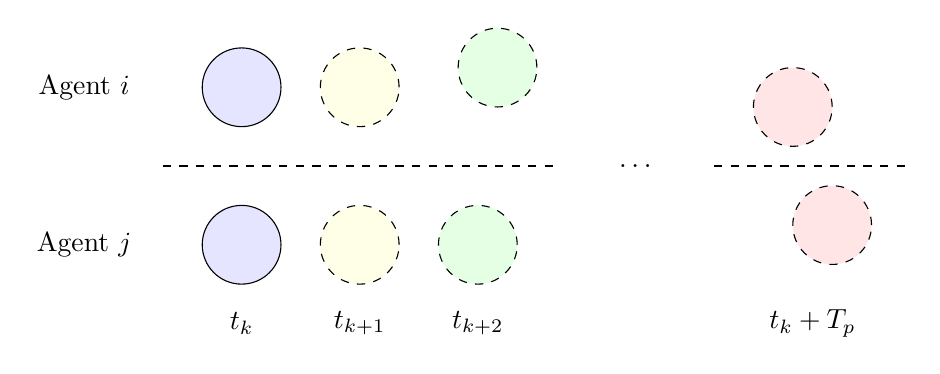
\begin{tikzpicture}[scale = 0.5]

  \draw[dashed] (0,0) -- (10,0);

  \node at (-2, 2) {Agent $i$};
  \node at (-2, -2) {Agent $j$};

  \filldraw[fill=blue!10!white, draw=black](2,2) circle (1cm);
  \filldraw[fill=blue!10!white, draw=black](2,-2) circle (1cm);
  \node at (2, -4) {$t_k$};


  \filldraw[fill=yellow!10!white, draw=black,dashed] (5,2) circle (1cm);
  \filldraw[fill=yellow!10!white, draw=black,dashed] (5,-2) circle (1cm);
  \node at (5, -4) {$t_{k+1}$};

  \filldraw[fill=green!10!white, draw=black,dashed] (8.5, 2.5) circle (1cm);
  \filldraw[fill=green!10!white, draw=black,dashed] (8,-2) circle (1cm);
  \node at (8, -4) {$t_{k+2}$};

  \node at (12, 0) {$\dots$};

  \draw[dashed] (14,0) -- (19,0);

  \filldraw[fill=red!10!white, draw=black,dashed] (16, 1.5) circle (1cm);
  \filldraw[fill=red!10!white, draw=black,dashed] (17,-1.5) circle (1cm);
  \node at (16.5, -4) {$t_k + T_p$};

\end{tikzpicture}

  \caption{The state of agent $i$ at each timestep is constrained by the state
    of $j$ at the same step.
    %Fully
    %outlined circles denote measured configurations, while partly outlined
    %circles denote predicted configurations. During the solution to the
    %individual optimization problems, the predicted configuration of each agent
    %at each timestep is constrained by the predicted configuration of the other
    %agent at the same timestep (hence the homologously identical colours at
    %each discrete timestep).
  }
  \label{fig:constraint_regime_horizon}
\end{figure}
\end{frame} %-------------------------------------------------------------------
\note{Now that agent $i$ knows where agent $j$ thinks he will move, we can
constrain the states of agent $i$ at each time step by the predicted state of
agent $j$ at the same time step. then, the constraint tightening takes care of
the rest.}
%###############################################################################
%###############################################################################
%###############################################################################
%###############################################################################
\begin{frame} %=================================================================
  \frametitle{Steering to the desired state}

  Remember\dots the designed control input $\vect{u}_i$ must\\[2ex]

  \begin{wideitemize}
    \item \textcolor{gray}{result in states that satisfy the state constraints} \\[2ex]
    \item drive trajectory to / stabilize at the desired state (how close?) \\[2ex]
    \item \textcolor{gray}{exist and be feasible $\forall t \geq 0$ ($\vect{u}_i \in \mathcal{U}_i$)} \\[2ex]
  \end{wideitemize}

\end{frame} %-------------------------------------------------------------------
\note{That takes care of the state feasibility. The question now is: how does
the input steer the state to the equilibrium?}
%###############################################################################
%###############################################################################
%###############################################################################
%###############################################################################
\begin{frame} %=================================================================
  \frametitle{Road-trip to equilibrium (1/7)}

\begin{figure}
  \scalebox{0.55}{\begin{tikzpicture}[scale = 1, rotate=-30]
  \draw (2,2) ellipse (6cm and 3cm);
    \node at ($(-3.8,0.8)+(75:6 and 3)$) {$\mathcal{E}_i$};
  \draw[dashed] (2,2) ellipse (5cm and 2.5cm);
    \node at ($(-2.3,1.2)+(75:5 and 2.5)$) {$\mathcal{E}_i \ominus \mathcal{B}_{i,t_{k+1} - t_k}$};
  \draw[dashed] (2,2) ellipse (4cm and 2cm);
    \node at ($(-1.3,1.1)+(75:4 and 2)$) {$\mathcal{E}_i \ominus \mathcal{B}_{i,t_{k+2} - t_k}$};
  \draw[dashed] (2,2) ellipse (2cm and 1cm);
    \node at ($(1.2,1.2)+(75:2 and 1)$) {$\mathcal{E}_i \ominus \mathcal{B}_{i,t_k + T_p - t_k}$};

  \node at (4.7,2) {$\dots$};
  \node at (-1,1.8) {$\dots$};

\pgflowlevel{\pgftransformrotate{30}}
\end{tikzpicture}
}
  \caption{Progressive tightening of the original constraint set $\mathcal{E}_i$.}
\end{figure}

\end{frame} %-------------------------------------------------------------------
\note{The constraint set tightening concludes at some set}
%###############################################################################
%###############################################################################
%###############################################################################
%###############################################################################
\begin{frame} %=================================================================
  \frametitle{Road-trip to equilibrium (2/7)}

\begin{figure}
  \scalebox{0.55}{\begin{tikzpicture}[scale = 1, rotate=-30]

  \draw[dashed](2,2) ellipse (5cm and 2.5cm);
    \node at ($(2.7,2.7)+(75:5 and 2.5)$) {$\mathcal{E}_i \ominus \mathcal{B}_{i,T_p}$};

  \pgflowlevel{\pgftransformrotate{30}}

\end{tikzpicture}
}
  \caption{The furthest the predicted trajectories must be restricted to: $\mathcal{E}_{i,t_k + T_p - t_k}$}
\end{figure}

\end{frame} %-------------------------------------------------------------------
\note{and suppose that this is it}
%###############################################################################
%###############################################################################
%###############################################################################
%###############################################################################
\begin{frame} %=================================================================
  \frametitle{Road-trip to equilibrium (3/7)}

\begin{figure}
  \scalebox{0.55}{\begin{tikzpicture}[scale = 1, rotate=-30]
  \draw[dashed](2,2) ellipse (5cm and 2.5cm);
    \node at ($(2.7,2.7)+(75:5 and 2.5)$) {$\mathcal{E}_i \ominus \mathcal{B}_{i,T_p}$};
  \draw[dashdotted](2,2) ellipse (4cm and 2cm);
    \node at ($(2.2,2.2)+(75:4 and 2)$) {$\Phi_i$};
\pgflowlevel{\pgftransformrotate{30}}
\end{tikzpicture}
}
  \caption{If linearized $g_i$ is stabilizable, there exists $\overline{\vect{e}}_i \in \Phi_i$: $\vect{u}_i = h(\overline{\vect{e}}_i) \in \mathcal{U}_i$.}
\end{figure}

\end{frame} %-------------------------------------------------------------------
\note{if this set is not empty, and if the linearized model of the system
is stabilizable, then we can find a feasible input whose form is linear
feedback with respect to the state, which}
%###############################################################################
%###############################################################################
%###############################################################################
%###############################################################################
\begin{frame} %=================================================================
  \frametitle{Road-trip to equilibrium (4/7)}

\begin{figure}
  \scalebox{0.55}{\begin{tikzpicture}[scale = 1, rotate=-30]
  \draw[dashed](2,2) ellipse (5cm and 2.5cm);
    \node at ($(2.7,2.7)+(75:5 and 2.5)$) {$\mathcal{E}_i \ominus \mathcal{B}_{i,T_p}$};
  \draw[dashdotted](2,2) ellipse (4cm and 2cm);
    \node at ($(2.2,2.2)+(75:4 and 2)$) {$\Phi_i$};
  \draw[dashdotted] (2,2) ellipse (3cm and 1.5cm);
    \node at ($(2.2,2.2)+(75:3 and 1.5)$) {$\Psi_i$};
\pgflowlevel{\pgftransformrotate{30}}
\end{tikzpicture}
}
  \caption{If this $\vect{u}_i$ is applied to a state in $\Psi_i$...}
\end{figure}

$\Psi_i = \{\vect{e}_i \in \mathcal{E}_i : V_i(\vect{e}_i) = \vect{e}_i^{\top} \mat{P} \vect{e}_i \leq \varepsilon_{\Psi_i},\ \ \varepsilon_{\Psi_i} > 0 \}$
\end{frame} %-------------------------------------------------------------------
\note{if we apply it to a state that lives in a set $\Psi$}
%###############################################################################
%###############################################################################
%###############################################################################
%###############################################################################
\begin{frame} %=================================================================
  \frametitle{Road-trip to equilibrium (5/7)}

\begin{figure}
  \scalebox{0.55}{\begin{tikzpicture}[scale = 1, rotate=-30]
  \draw[dashed](2,2) ellipse (5cm and 2.5cm);
    \node at ($(2.7,2.7)+(75:5 and 2.5)$) {$\mathcal{E}_i \ominus \mathcal{B}_{i,T_p}$};
  \draw[dashdotted](2,2) ellipse (4cm and 2cm);
    \node at ($(2.2,2.2)+(75:4 and 2)$) {$\Phi_i$};
  \draw[dashdotted] (2,2) ellipse (3cm and 1.5cm);
    \node at ($(2.2,2.2)+(75:3 and 1.5)$) {$\Psi_i$};
  \draw (2,2) ellipse (2cm and 1cm);
    \node at ($(2.2,2.2)+(75:2 and 1)$) {$\Omega_i$};
\pgflowlevel{\pgftransformrotate{30}}
\end{tikzpicture}
}
  \caption{If this $\vect{u}_i$ is applied to a state in $\Psi_i$, the
    resulting state will end up in $\Omega_i$.}
\end{figure}

$\Omega_i = \{\vect{e}_i \in \mathcal{E}_i : V_i(\vect{e}_i) = \vect{e}_i^{\top} \mat{P} \vect{e}_i \leq \varepsilon_{\Omega_i},\ \ \varepsilon_{\Omega_i} \in (0, \varepsilon_{\Psi_i})  \}$
\end{frame} %-------------------------------------------------------------------
\note{it will move the state to the terminal set}
%###############################################################################
%###############################################################################
%###############################################################################
%###############################################################################
\begin{frame} %=================================================================
  \frametitle{Road-trip to equilibrium (6/7)}

\begin{figure}
  \scalebox{0.55}{\begin{tikzpicture}[scale = 1, rotate=-30]
  \draw[dashed](2,2) ellipse (5cm and 2.5cm);
    \node at ($(2.7,2.7)+(75:5 and 2.5)$) {$\mathcal{E}_i \ominus \mathcal{B}_{i,T_p}$};
  \draw[dashdotted](2,2) ellipse (4cm and 2cm);
    \node at ($(2.2,2.2)+(75:4 and 2)$) {$\Phi_i$};
  \draw[dashdotted] (2,2) ellipse (3cm and 1.5cm);
    \node at ($(2.2,2.2)+(75:3 and 1.5)$) {$\Psi_i$};
  \draw (2,2) ellipse (2cm and 1cm);
    \node at ($(2.2,2.2)+(75:2 and 1)$) {$\Omega_i$};
\pgflowlevel{\pgftransformrotate{30}}
\end{tikzpicture}
}
  \caption{Once inside $\Omega_i$, the trajectory is trapped there ($\Omega_i$ is invariant).}
\end{figure}



\end{frame} %-------------------------------------------------------------------
\note{and since $\Omega$ is a subset of $\Psi$, it will always stay inside $\Omega$.}
%###############################################################################
%###############################################################################
%###############################################################################
%###############################################################################
\begin{frame} %=================================================================
  \frametitle{Road-trip to equilibrium (7/7)}

\begin{figure}
  \scalebox{0.55}{\begin{tikzpicture}[scale = 1, rotate=-30]
  \draw[dashed](2,2) ellipse (5cm and 2.5cm);
    \node at ($(2.7,2.7)+(75:5 and 2.5)$) {$\mathcal{E}_i \ominus \mathcal{B}_{i,T_p}$};
  \draw[dashdotted](2,2) ellipse (4cm and 2cm);
    \node at ($(2.2,2.2)+(75:4 and 2)$) {$\Phi_i$};
  \draw[dashdotted] (2,2) ellipse (3cm and 1.5cm);
    \node at ($(2.2,2.2)+(75:3 and 1.5)$) {$\Psi_i$};
  \draw (2,2) ellipse (2cm and 1cm);
    \node at ($(2.2,2.2)+(75:2 and 1)$) {$\Omega_i$};
\pgflowlevel{\pgftransformrotate{30}}
\end{tikzpicture}
}
  \caption{Once inside $\Omega_i$, the trajectory is trapped there ($\Omega_i$ is invariant).}
\end{figure}

Provided that $\overline{\delta}_i \leq \xi(\varepsilon_{\Psi_i} - \varepsilon_{\Omega_i}, T_p)$, $\xi(\nearrow, \searrow)$,
the trajectory never escapes $\Omega_i$.


\end{frame} %-------------------------------------------------------------------
\note{the size of the terminal set depends on the how strong the disturbance is
and on the hierarchy of all of these sets. Provided that the supremum is
bounded by a certain threshold that depends on the size of the terminal set and
$\Psi$, and the length of the horizon.}
%###############################################################################
%###############################################################################
%###############################################################################
%###############################################################################
\begin{frame} %=================================================================
  \frametitle{Recursive feasibility}

  Remember\dots the designed control input $\vect{u}_i$ must\\[2ex]

  \begin{wideitemize}
    \item \textcolor{gray}{result in states that satisfy the state constraints} \\[2ex]
    \item \textcolor{gray}{drive the trajectory / stabilize at the desired state (how close?)} \\[2ex]
    \item exist and be feasible $\forall t \geq 0$ ($\vect{u}_i \in \mathcal{U}_i$) \\[6ex]
  \end{wideitemize}

  Can show that

  \textit{if the solution is feasible at $t=0$, then there are past controls
  and an auxiliary feedback controller $\forall t > 0$, both in $\mathcal{U}_i$}.
\end{frame} %-------------------------------------------------------------------
\note{as for the feasibility of the input, we can patch together past control
sequences with the feedback controller and come up with a feasible control signal}
%###############################################################################
%###############################################################################
%###############################################################################
%###############################################################################
\begin{frame} %=================================================================
  \frametitle{Solution requirements (III/III): stabilization}

  Design decentralized control policies $\vect{u}_i \in \mathcal{U}_i$ such that\\[3ex]

  \begin{wideitemize}

    \item Collisions are avoided for all\ \ $i,j \in \mathcal{V}$,\ \ $\ell \in \mathcal{L}$,\ \ $t \geq 0$
      \begin{align}
        \|\vect{p}_i(t) - \vect{p}_{j}(t)\| > \underline{d}_{ij,a} \\
        \|\vect{p}_i(t) - \vect{p}_\ell\| > \underline{d}_{i\ell,o}
      \end{align}

      $\vect{p}_i$ component of state $\vect{x}_i$\\[3ex]

    \item Neighbours $i \in \mathcal{N}_j$, $j \in \mathcal{N}_i$
      maintain connectivity at all times $t \geq 0$
      \begin{align}
        \|\vect{p}_i(t) - \vect{p}_{j}(t)\| < \text{min}(\overline{d}_{i}, \overline{d}_{j})
      \end{align}

  \end{wideitemize}

  \begin{gg_box}
  \begin{wideitemize}
    \item (Closed-loop) System is stable at desired state
      \begin{align}
        \lim\limits_{t \to \infty}\|\vect{x}_i(t) - \vect{x}_{i,\text{des}}\| \to 0 \\
      \end{align}
  \end{wideitemize}

  \end{gg_box}

\end{frame} %-------------------------------------------------------------------
\note{Now the last thing is the actual stabilization.}
%###############################################################################
%###############################################################################
%###############################################################################
%###############################################################################
\begin{frame} %=================================================================
  \frametitle{How is stabilization achieved?}

     \begin{align}
       \lim\limits_{t \to \infty}\|\vect{x}_i(t) - \vect{x}_{i,\text{des}}\| \ \  \textcolor{red}{\xcancel{\to}} \ \ 0 \\[4ex] \\
       \vect{e}_i^{\top} \mat{P} \vect{e}_i \leq \varepsilon_{\Omega_i}
      \end{align}

\end{frame} %-------------------------------------------------------------------
\note{it turns out that we cannot drive the system to complete equilibrium, but
  we can only trap it in a neighbourhood of it. this neighbourhood is smaller
than that which it would have been if the controller didn't manage to
attenuate the disturbances.}
%###############################################################################
%###############################################################################
%###############################################################################
%###############################################################################
\begin{frame} %=================================================================
  \frametitle{How is stabilization achieved?}

  Can be shown that the optimal cost $J_i^{\star} = J_i\big(\vect{e}_i, \overline{\vect{u}}_i^{\star}\big)$\\[2ex]
  is an \textit{Input-to-state} Lyapunov function in $\mathcal{E}_i$ for all $\vect{\delta}_i: \|\vect{\delta}_i\|_{\infty} \leq \overline{\delta}_i$\\[4ex]

  In essence: \\
  \begin{wideitemize}
    \item the \textit{trajectory} is bounded in $\Omega_i$: it does not escape $\Omega_i$\\[2ex]
    \item the \textit{desired state} is not  asymptotically stable unless the disturbance is decaying
  \end{wideitemize}

\end{frame} %-------------------------------------------------------------------
\note{We can show that the cost that results from the application of the
suggested control input, the optimal cost, rather than monotonically deacreasing,
is bounded. In this case we can prove that the optimal cost is an input-to-state
lyapunov function, which makes the closed-loop system input-to-state stable
within its constraints set}
%###############################################################################
%###############################################################################
%###############################################################################
%###############################################################################
\begin{frame} %=================================================================
  \begin{center}
    Simulations
  \end{center}
\end{frame} %-------------------------------------------------------------------
%###############################################################################
%###############################################################################
%###############################################################################
%###############################################################################
\begin{frame} %=================================================================
  \frametitle{Example system: the unicycle}

\begin{minipage}{0.45\textwidth}
  Unicycle dynamics

  \begin{align}
    \dot{x}_i(t) &= v_i(t) \cos\theta_i(t) + \delta_i(t)\\[2ex]
    \dot{y}_i(t) &= v_i(t) \sin\theta_i(t) + \delta_i(t)\\[2ex]
    \dot{\theta}_i(t) &= \omega_i(t) + \delta_i(t)\\[4ex]
    \delta_i(t) &= \overline{\delta}_i \sin2t
  \end{align}
\end{minipage} \hfill
\begin{minipage}{0.4\textwidth}
  States: $x_i$, $y_i$, $\theta_i$\\[2ex]
  Inputs: $v_i$, $\omega_i$\\[2ex]
  Disturbance: $\overline{\delta}_i = 0.1$\\[2ex]
  $i \in \{1,2,3\}$\\[2ex]
\end{minipage}

\end{frame} %-------------------------------------------------------------------
\note{From this point on I will only show you how the control regime that I
have described to you performs in simulations. We will use the standard
unicycle model moving in $x-y$ and rotating around the $z$ axis. Its states
are $xy\theta$ and its inputs are the longitudinal velocity and the
angular velocity}
%###############################################################################
%###############################################################################
%###############################################################################
%###############################################################################
\begin{frame} %=================================================================
  \frametitle{Simulation example I/II: 2D Trajectories}

\leavevmode\hidewidth
\begin{center}
\begin{tikzpicture}[remember picture]
   \node[anchor=south west, inner sep=0pt] at (current page.south east) {%
   %\node[anchor=south west, inner sep=0pt] at (0.1\paperwidth,0.1\paperheight) {
     \movie[height = 0.5\paperheight, width = 0.72\paperwidth, poster, showcontrols, autostart,loop] {}{figures/trajectories_thorough_lossless.avi}%
   };
\end{tikzpicture}
\end{center}

2D trajectories of agent 1 (blue, middle), agent 2 (yellow, below)
and agent 3 (red, above). Black circles are obstacles. Agents 2 and 3 must
keep connectivity with agent 1. Disturbances are absent. Trajectories with
and without disturbances are more or less similar. Only steady-state changes.
\leavevmode\hidewidth

\end{frame} %-------------------------------------------------------------------
\note{Here we see three agents trying to get to their desired positions marked
with x, that have to bypass these two obstacles. The blue one needs to be within
certain bounds from the other two, and they all must not hit the obstacles or
each other.}
%###############################################################################
%###############################################################################
%###############################################################################
%###############################################################################
\begin{frame} %=================================================================
  \frametitle{Simulation example II/II: Equilibrium close-up}

\leavevmode\hidewidth
\begin{center}
\begin{tikzpicture}[remember picture]
   \node[anchor=south west, inner sep=0pt] at (current page.south east) {%
   %\node[anchor=south west, inner sep=0pt] at (0.1\paperwidth,0.1\paperheight) {
     \movie[height = 0.5\paperheight, width = 0.72\paperwidth, poster, showcontrols, autostart,loop] {}{figures/terminal_OFF_OM.avi}%
   };
\end{tikzpicture}
\end{center}

The effect of unattenuated disturbances on the steady-state
configurations. Left: no disturbance. Right: unattenuated additive bounded
disturbances with $\overline{\delta}_i = 0.1$.
\leavevmode\hidewidth

\end{frame} %-------------------------------------------------------------------
\note{If we look at what happens around the desired equilibrium, we see on the
left that we can totally stabilize the system when there are no disturbances.
On the righthand side we see the effect of disturbances which have a supremum
of $0.1$, that have not been attenuated to the trajectories of the systems
around the equilibrium.}
%###############################################################################
%###############################################################################
%###############################################################################
%###############################################################################
\begin{frame} %=================================================================
  \frametitle{Simulation example II/II: Equilibrium close-up}

\leavevmode\hidewidth
\begin{center}
\begin{tikzpicture}[remember picture]
   \node[anchor=south west, inner sep=0pt] at (current page.south east) {%
   %\node[anchor=south west, inner sep=0pt] at (0.1\paperwidth,0.1\paperheight) {
     \movie[height = 0.5\paperheight, width = 0.72\paperwidth, poster, showcontrols, autostart,loop] {}{figures/terminal_OFF_OM_ON.avi}%
   };
\end{tikzpicture}
\end{center}
Steady-state configurations. Left: no disturbance. Middle: unattenuated additive
bounded disturbances with $\overline{\delta}_i = 0.1$. Right: attenuated
additive bounded disturbances with $\overline{\delta}_i = 0.1$ as a result
of the proposed control regime.
\leavevmode\hidewidth

\end{frame} %-------------------------------------------------------------------
\note{if we design the control system the way i described you here today, then
we can make the system get closer to its desired state.}
%###############################################################################
%###############################################################################
%###############################################################################
%###############################################################################
\begin{frame} %=================================================================
  \frametitle{Conclusion}
  It is possible to design a feasible control regime based on the principle of
  Receding Horizon Control such that, a multi-agent system constrained with
  connectivity and collision constraints on the states and input constraints,
  is stable under the influence of disturbances.
\end{frame} %-------------------------------------------------------------------
\note{It is possible to design a feasible control regime based on the principle of
  Receding Horizon Control such that, a multi-agent system constrained with
  connectivity and collision constraints on the states and input constraints,
  is stable under the influence of disturbances.}
%###############################################################################
%###############################################################################
%###############################################################################
%###############################################################################
\begin{frame} %=================================================================
  \begin{center}
  Thank you for your attention.
  \end{center}
\end{frame} %-------------------------------------------------------------------

%\begin{frame} %=================================================================
%\end{frame} %-------------------------------------------------------------------

%\begin{frame} %=================================================================
%\end{frame} %-------------------------------------------------------------------

%\begin{frame} %=================================================================
%\end{frame} %-------------------------------------------------------------------

%\begin{frame} %=================================================================
%\end{frame} %-------------------------------------------------------------------
